\chapter{Implementation}\label{ch:implementation}

The previous sections explained \textit{what} the application should do, which goals should be achieved and which requirements we surely want the application meets. In this section, more details are provided about \textit{how} all this is translated to the implementation.

\section{Design Choice}
Before we started with the actual implementation, we had to decide how to achieve the first research goal, i.e. how will we make sure the application is devide- and OS-independent? A first technique could have been to make use of the Java Virtual Machine. This approach would work but at least one big problem comes along with it. We want to make it possible to let multiple people work on the same visualization, eventually at the same time. Therefore, it is more convenient to have a browser-based application. A browser is device- and OS-independent and lots of technologies exist to create applications and visualizations for the web.

% --------------------
% --- TECHNOLOGIES ---
% --------------------
\section{Technologies}\label{sec:technologies}
A number of technologies assisted in the developing process of the application. In this section, each of these technologies is discussed to explain its importance.

\subsection{ReactJS}\label{sec:reactjs}
ReactJS is an open source library to create user interfaces\footnote{\url{https://reactjs.org/index.html}}. One of its main goals is to provide the best possible rendering performances\footnote{\url{https://medium.com/@thinkwik/why-reactjs-is-gaining-so-much-popularity-these-days-c3aa686ec0b3}}. Performance is high because ReactJS allows developers to break down the user interface into different components. Each component has its own \textit{state}, which contains information about the content of the component. This state can be updated while the application is running and if such an update is made, only this component is re-rendered instead of re-rendering the complete UI\footnote{\url{https://facebook.github.io/react/docs/why-react.html}}. Hence, this involves a huge benefit for the performance. Next to that, it is also not very hard to learn to code in React when comparing to other frameworks (e.g. AngularJS). If the developer knows HTML and JavaScript, he will be able to code in ReactJS quickly.\\

Because of these benefits, ReactJS is the framework in which the GuideaMaps application is implemented. Each node is considered as a separate and unique React Component. The most important reason for implementing the nodes like this is performance: if the state of the node is updated, only this node is re-rendered and not the complete UI.

\subsection{d3}\label{sec:d3}
Another helpful tool is d3. With d3-hierarchy\footnote{\url{https://github.com/d3/d3-hierarchy}}, it is possible to transform JSON-data into hierarchical data. Having this kind of data makes it much easier to create a tree- or cluster-structure. In the case of GuideaMaps, a clustered visualization is very useful. The \textit{main}-node (a.k.a. the root node) is then positioned at the center, such that its child nodes can be placed around it. Hence, the farther a node is away from the center, the lower it is in the hierarchy. Also, the visualization will not be messed up by positioning the nodes in this way, because every node has exactly one parent. This means there won't be a spaghetti of links where you cannot see which node the link comes from and which node it is pointing to.

\subsection{Tailwind CSS}\label{sec:tailwind}
The style of the application is very important for the end user. Everything should look pretty and, as already mentioned in section \ref{sec:usability-requirements}, the possibilities should be straightforward and visible. While developing and creating a beautiful style for applications and websites, the code for these styles can become a big part of the implementation. Hence, a good framework is necessary to reduce the lines of style code to a reasonable number. It also helps to improve the readability of the code.\\

Tailwind CSS\footnote{\url{https://tailwindcss.com/}} is a framework that assists developers to style their application. The difference with more famous frameworks, like Bootstrap, is that Tailwind CSS has no default theme. If you want to use a Bootstrap-feature, this eventually comes along with other features you don't always wanted and it can be quite hard to undo the part you didn't ask for. With tailwind on the other hand, you can grab only the features you want, without side-effects. Figure \ref{fig:examplecode-tailwindcss} shows an example with two small listings. The first uses inline style while the second makes use of tailwind CSS.\\

\begin{figure}[H]
	\begin{minipage}[b]{0.5\textwidth}
 		\centering
  		\begin{minted}[linenos, escapeinside=||]{html}
<div
  style={{
    position: absolute|,|
    border: 1px solid black|,|
    borderRadius: O.25rem|,|
    padding: 0.5rem|,|
  }}
/>
		\end{minted}
		\label{lst:no-tailwind}
		\captionof{lstlisting}{Normal CSS, no tailwind.}
	\end{minipage}
 	\begin{minipage}[b]{0.5\textwidth}
  		\centering
		\begin{minted}[breaklines, escapeinside=||]{html}
<div
    className={
      |'|absolute border border-solid border-black rounded p-2|'|
    }
/>
		\end{minted}
		\label{lst:tailwind}
 	 	\captionof{lstlisting}{With tailwind CSS.}
 	\end{minipage}
	\caption{Difference when using tailwind CSS or not.}
	\label{fig:examplecode-tailwindcss}
\end{figure}

The figure illustrates the difference to implement four css property-value pairs in normal css and implementing the same four with tailwind. In the case of normal css, we need four lines of code to retrieve the intended result. On the other hand, with tailwind css, we add some classes providing the same style. The classnames can be placed on a single line instead of four. This example proves that the number of lines can be decreased.





% ---------------------
% ----- STRUCTURE -----
% ---------------------
\section{Main Code Structure}\label{sec:structure}
With the technologies mentioned in the previous section, the most important pillars the application relies on are discussed. In this section, we will explain the main structure of the code, such that it is clear how all elements work together. Figure \ref{fig:overall-structure} shows a visualization of the structure of the code.
\begin{figure}[H]
	\centering
	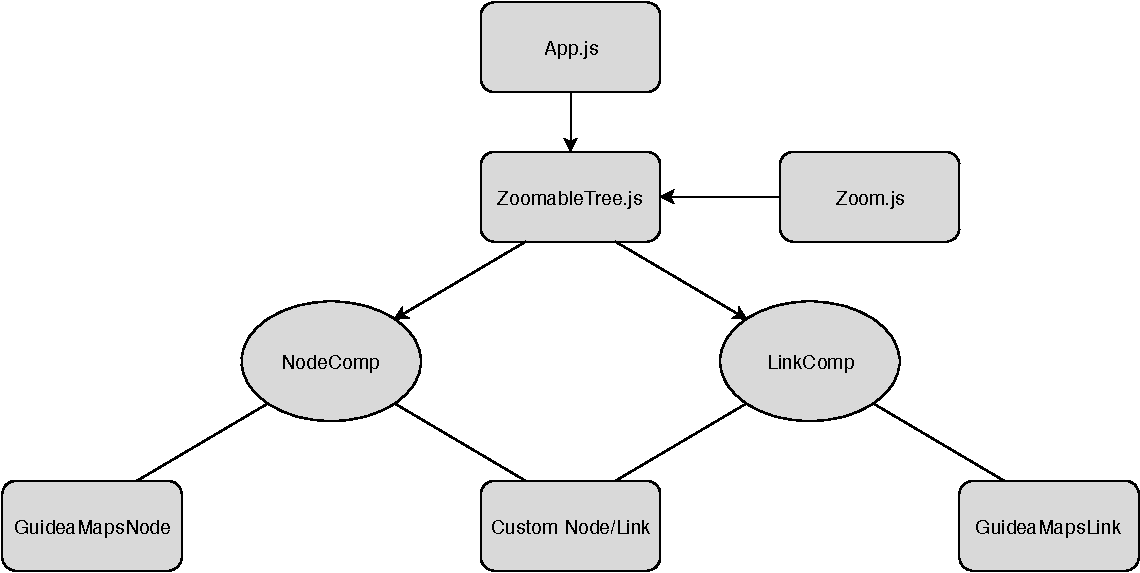
\includegraphics[width=\linewidth]{thesis-architecture.pdf}
	\caption{Structure of the application.}
	\label{fig:overall-structure}
\end{figure}

The application is developed in such a way that it can be used as a library for other purposes than GuideaMaps as well. Hence, the research goal to have a generic solution is achieved. The general, always-returning part of the code can be found in App.js, ZoomableTree.js and Zoom.js, where the layout of the nodes is defined as well as the implementation to allow the user to zoom the visualization in and out. When talking about the library, the layer of the NodeComp and LinkComp is very interesting and important. For the GuideaMaps, an implementation for a GMNode and GMLink is provided. Each implementation describes what every node and every link should look like in the visualization.\\

The strength of the library can not only be seen at its genericity but also when a particular user would like to have a different representation for the nodes or the links or both. In that case, new components (e.g. MyCustomNode and MyCustomLink) should be implemented. In the code, only one line should be adapted: in App.js, ZoomableTree is called with a certain number of props. Two of these props are NodeComp and LinkComp, which are set to GMNode and GMLink, respectively, by default. Hence, the only action that is required to \textit{plug in} an other component is replacing GMNode by MyCustomNode and GMLink by MyCustomLink. Hence, the visualization can be customized to the needs of the user. Figure \ref{fig:examplecode-library} shows the part of the code in App.js that should be adapted as explained. Note that NodeComp and LinkComp are not the only props that are passed to ZoomableTree. The others are omitted to improve the readability.

\begin{figure}[H]
	\begin{minipage}{0.5\textwidth}
 		 \centering
		 \begin{minted}[linenos]{html}
<ZoomableTree
    NodeComp={GMNode}
    LinkComp={GMLink}
/>
		\end{minted}
		\label{lst:default-components}
		\captionof{lstlisting}{Default components.}
	\end{minipage}
 	\begin{minipage}{0.5\textwidth}
  		\centering
  		\begin{minted}{html}
<ZoomableTree
    NodeComp={MyCustomNode}
    LinkComp={MyCustomLink}
/>
		\end{minted}
		\label{lst:custom-components}
 	 	\captionof{lstlisting}{Custom components.}
 	\end{minipage}
	\caption{Two listings showing how to use the library.}
	\label{fig:examplecode-library}
 	%\captionof{figure}{Two listings showing the difference between the default and custom use of the library.}
\end{figure}





% ------------------------------
% ----- GUIDEAMAPS DETAILS -----
% ------------------------------
\section{Default Implementation: GuideaMaps}
Now the overview of the structure of the application is discussed, we will consider the GuideaMaps visualization and its implementation details in this section. The resulting visualization can be seen in figure \ref{fig:guideamaps}.
 
\begin{figure}[H]
	\centering
	\frame{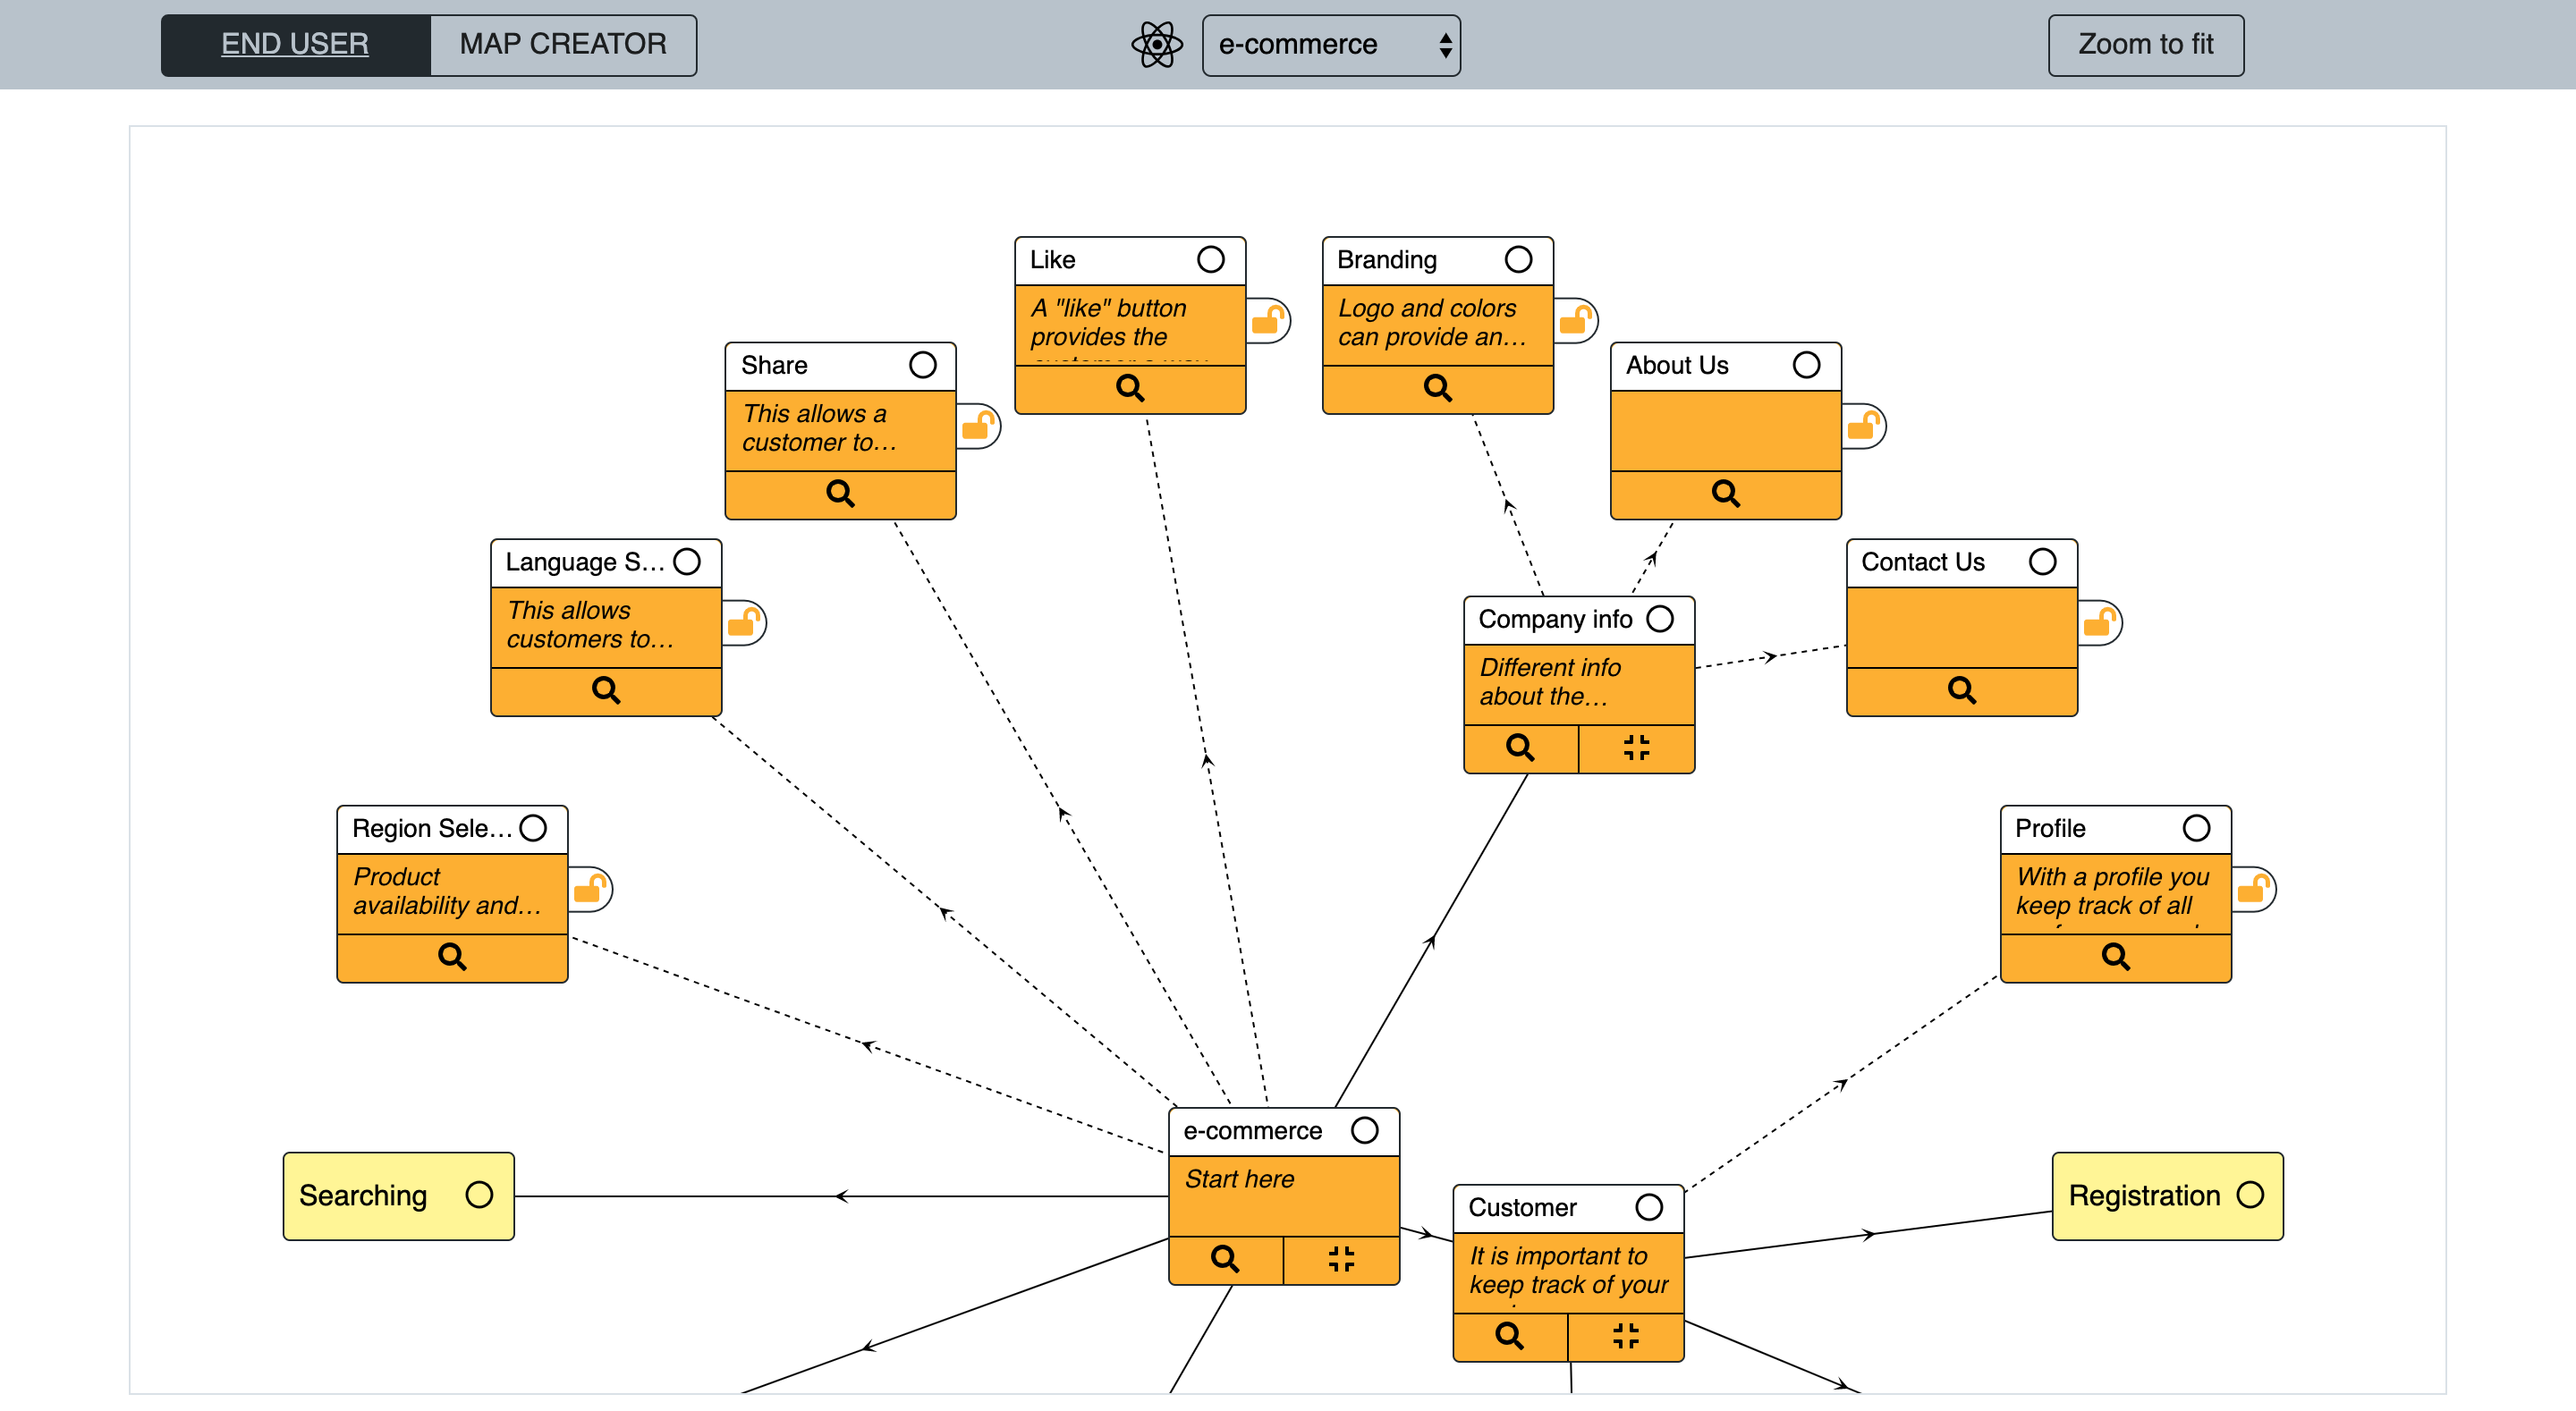
\includegraphics[width=\linewidth]{guideamaps.png}}
	\caption{GuideaMaps Layout.}
	\label{fig:guideamaps}
\end{figure}

The nodes represent a specific part of the data and the links illustrate the relation between the data (i.e. the nodes). Before we discuss the nodes into detail, we start with the \textit{navigation bar} above the visualization itself. This navigation bar is divided in three equal parts. In the center, the user can select which visualization he wants to use via an option menu. The name of the currently selected option is always visible. There are several reasons why this is possible. The first is because the user should be able to switch between templates. A user should not be limited to one possible visualization. As a map creator, you can create a new template, which then can be filled with data by the end users. As an end user, you should be able to switch between different visualizations because it is possible that you are working on more than one visualization at the same time.\\

The right part of the navigation bar contains a single button. A click on this button makes sure the visualization is zoomed to a certain level where all nodes fit on the screen. This is one of the reasons why we mentioned in the requirements (section \ref{sec:other-requirements}) that the screen of the used device should not be too small.\\

The left part is created to be able to switch between the user roles \textcolor{red}{or modes???} (i.e. end user or map creator). A map creator has more rights and hence he can perform more actions than an end user. In the following subsections, the differences between these roles \textcolor{red}{or modes???} is elaborated.

\begin{figure}[H]
	\centering
	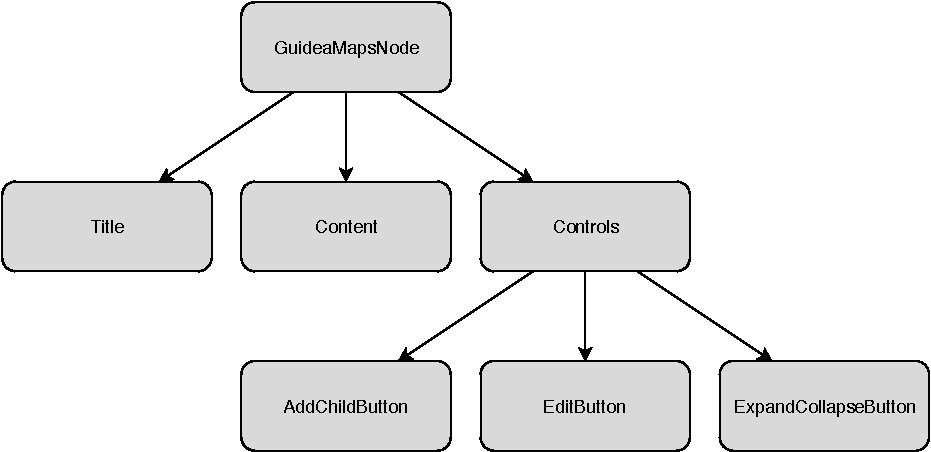
\includegraphics[width=\linewidth]{GMStructure.pdf}
	\caption{Structure of GuideaMapsNode.}
	\label{fig:gmnodestructure}
\end{figure}

As you can see in figure \ref{fig:gmnodestructure}, the structure of a GuideaMapsNode node is quite easy. Each node consists of three html \textit{div}-elements: a title-div, a content-div and a controls-div.

\addtocontents{toc}{\protect\setcounter{tocdepth}{1}} % hide the following subsections from the table of contents
\subsection{Title}
The title-div is positioned at the top of the node. It consists of the title text when this is given by the map creator. Otherwise, it shows \textit{Insert title} in italics to remind the user that he still had to set a title for this node. An end user can set the title if no title exists yet, but he can never change it. The reason for this is because we distinguish two situations. In the first situation, the end user adds a child node for a particular parent. This node has not title by default and then he should be able to insert a title. In the second situation, the user opens an existing node created by the map creator. In that case an end user is not allowed to change the title of the node, because otherwise he would be able to change the complete layout of the visualization. \\

Next to the title-text, the title-div contains an icon placed near the right border. This icon indicates whether all information, i.e. some content, is provided or not. The icon that is shown also depends on whether the information in its child-nodes is filled in or not. We distinguish three possible situations:
\begin{enumerate}
	\item The data of the node itself and of all of its children are correctly filled in. In this case the icon will be a completely filled circle.
	\item The data of the node itself and of all of its children are all empty. In this case the icon will be an empty circle.
	\item In all other cases, the data of the node itself or of at least one of its nodes is filled in. Then the icon will be a semi-filled circle.
\end{enumerate}
This icon can assist the user in determining whether all information is filled in. For example, if he checks the root node and sees that the circle is completely filled, he does not have to check every child-node to know that all information is filled in. On the other hand, suppose only one node is not yet provided of some content. If the user then starts from the root node and always follows the child-node with a semi-filled circle, he will find the incomplete node much faster than in the case he has to check all the nodes.



\subsection{Content}
The content of each node is just some text describing the information corresponding to the title. As long as no content is provided by the user, a description is shown in italics to instruct the user which content to provide.



\subsection{Controls}
The last part of a node is the controls-div. With \textit{controls} we mean the different actions that a user can take concerning the particular node. The controls consist of three buttons: one to add a child node, one to ``open'' the node to view and edit the data and one to expand or collapse the node to show or hide the child nodes, respectively. When a node is collapsed, all child nodes on all lower levels in the hierarchy are hidden. On the other hand, when a node is expanded, only the child-nodes of the next level in the hierarchy are shown.



\subsection{EditModal}
A click on the button to open the node opens a modal representing the data. What this modal looks like depends on the mode. If we are in map creator mode, a form will be shown to allow to change the title, the description, the content itself and the background color. In the case of the end user mode, only the content and the background color can be changed. Only the first time a child node is added and no title and description is filled in yet, the end user is able to fill in these data as well.\\

When changing the background color, the user can choose to include all children or not. If the checkbox ``include children'' is checked, the background color of all child-nodes on all sublevels in the hierarchy will be changed to the new color. Otherwise, only the background color of the current node will be changed.\\

The text color is black by default. This can become a problem when the background color is changed to a dark color and certainly when it is black as well because then the text is not readable anymore. To solve this issue, we wrote some CSS rules that change the text-color depending on the background color. A black (or dark) background will result in white text and a white (or light) background results in black text.
 


\subsection{Optional nodes}
The visualization also provides optional nodes. They can be recognized by the link between this node and its parent. A regular node is connected to its parent via a solid link, while an optional node is connected via a dashed link. A special characteristic is that these nodes can be disabled by the end user. Optional nodes contain an additional button at their right side with a lock. As long as the node is enabled, the button is represented by an open lock. A click on this button disables the node and changes the icon to a closed lock. A second click re-enables the node. Next to the lock icon, a disabled node can be recognized by its gray background and a blur so that you cannot see the content anymore.
\addtocontents{toc}{\protect\setcounter{tocdepth}{2}} % add the following subsections again to the table of contents














